\documentclass[tikz,border=10pt]{standalone}
\usepackage{amsmath}
\usetikzlibrary{angles,quotes}
\begin{document}
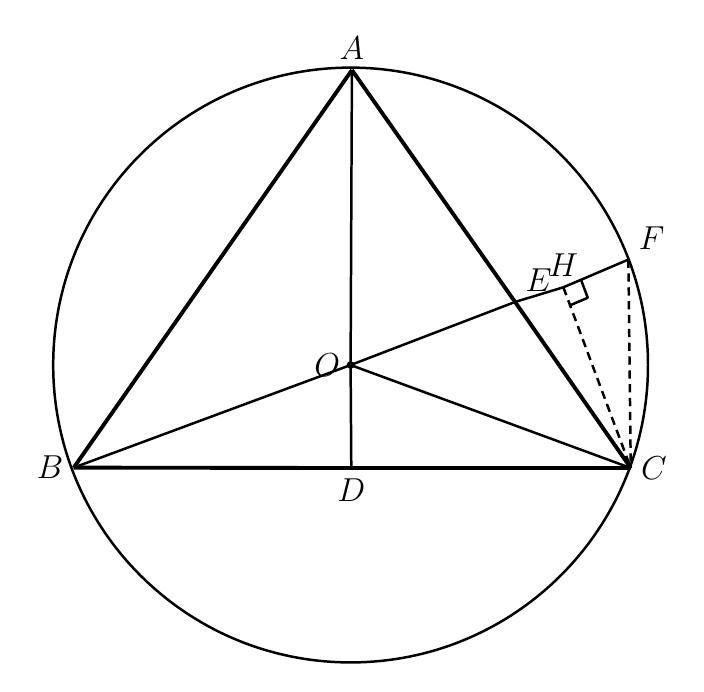
\begin{tikzpicture}[line join=round, line width=0.9pt,
  lbl/.style={font=\fontsize{11.5}{13.8}\selectfont},
  dashedge/.style={dash pattern=on 3pt off 2pt}]
\coordinate (A) at (-0.008,3.492);
\coordinate (B) at (-3.541,-1.557);
\coordinate (C) at (3.533,-1.562);
\coordinate (D) at (-0.016,-1.562);
\coordinate (E) at (2.064,0.547);
\coordinate (F) at (3.503,1.085);
\coordinate (H) at (2.677,0.733);
\coordinate (O) at (-0.025,-0.254);












\draw (O) circle[radius=3.777];


\draw[line width=1.4pt] (A) -- (B);
\draw[line width=1.4pt] (A) -- (E) -- (C);
\draw[line width=1.4pt] (B) -- (D) -- (C);


\draw (A) -- (O) -- (D);


\draw (B) -- (O) -- (E) -- (H) -- (F);


\draw (C) -- (O);


\draw[dashedge] (F) -- (C);
\draw[dashedge] (H) -- (C);


\draw pic[draw, angle radius=0.244cm] {right angle=F--H--C};

\fill (O) circle (1.400pt);


\node[lbl, above] at (A) {$A$};
\node[lbl, left] at (B) {$B$};
\node[lbl, right] at (C) {$C$};
\node[lbl, below] at (D) {$D$};
\node[lbl, above right] at (E) {$E$};
\node[lbl, above right] at (F) {$F$};
\node[lbl, above] at (H) {$H$};
\node[lbl, left] at (O) {$O$};
\end{tikzpicture}
\end{document}